%%%%%%%%%%%%%%%%%%%%%%%
% Binghampton Pre-Talk
%%%%%%%%%%%%%%%%%%%%%%%



% Title Page
{
%\setbeamercolor{background canvas}{bg=UniGray}
%\setbeamertemplate{title page}[default][colsep=-4bp,rounded=true,shadow=\beamer@themerounded@shadow]
%\setbeamertemplate{title page}[rounded=true,shadow=false]
\begin{frame}
\titlepage
\end{frame}
}



% Motivation
\begin{frame}[plain]
\begin{itemize}
\item Can a square and a cube of a rational number differ by 2: $x^2 - x^3= 2$

\item Can a square and a cube of rational numbers differ by 2: $y^2 - x^3= 2$

\item Are there right triangles with all three sides rational, and with rational area: $a^2+b^2=c^2$, $\dfrac{ab}{2}= N$. This naturally leads to rational points on $y^2= x^3 - n^2 x$

\item What numbers are the sum of two (or more) cubes: $x_1^3+x_2^3+\cdots+x_n^3= N$
\end{itemize}
\end{frame}




% Quote
{\setbeamertemplate{background canvas}{
\tikz[remember picture,overlay]
	\node[opacity=0.3] at (current page.center) {
	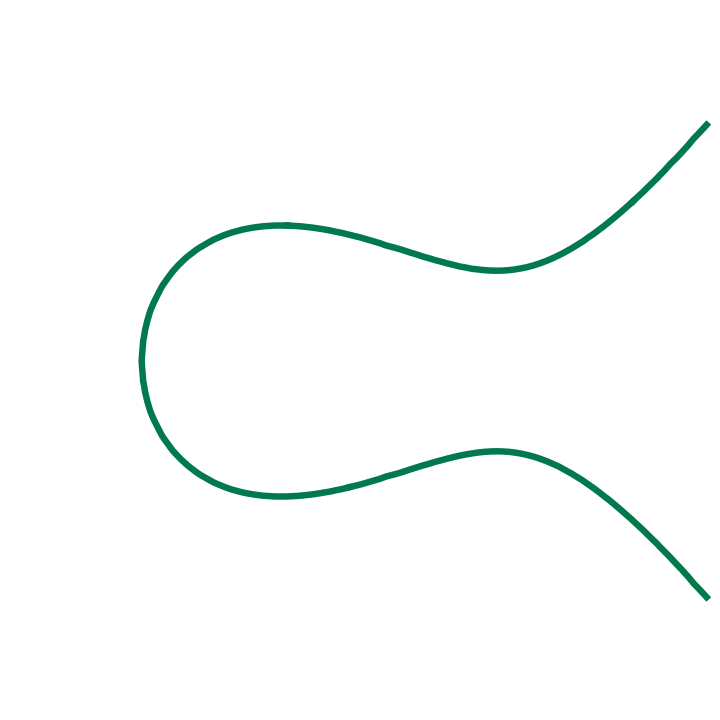
\includegraphics[width=\paperwidth,
	height=\paperheight]{images/curve.png}};} 
\begin{frame}[plain]
	\begin{minipage}{0.2\textwidth}
 	\begin{figure}[h]
	\centering
	\fbox{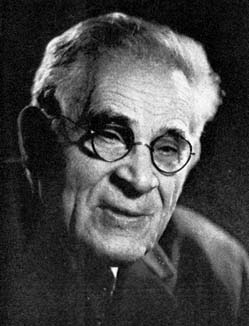
\includegraphics[width=1\textwidth]{images/mordell.jpg}} \par
	{\small 1888--1972}
	\end{figure}
	\end{minipage}%
	\begin{minipage}{0.8\textwidth}
	\begin{center}
	{\itshape ``Mathematicians have been familiar with very few questions for so long a period with so little accomplished in the way of general results, as that of finding the rational [points on elliptic curves].''} \\
	 \phantom{x}\hfill-- L.J. Mordell, 1922
	\end{center}
 	\end{minipage}
\end{frame}
}



% Introduction
\begin{frame}[plain]

\begin{ques}
Let $F(x_1,x_2,\ldots,x_n) \in \Q[x_1,\ldots,x_n]$. Consider the equation $F= 0$.
\begin{itemize}
\item When are there rational solutions?
\item If there are rational solutions, how many are there?
\item Can we find/parametrize all the rational solutions?
\item What about integer solutions?
\end{itemize}
\end{ques}
\end{frame}



% Hilbert's 10 Problem
\begin{frame}[plain]
\frametitle{\textcolor{white}{Hilbert's 10\textsuperscript{th} Problem}}

\begin{table}[!ht]
\begin{tabular}{|c|c|c}  \cline{1-2}
Ring & Hilbert's 10\textsuperscript{th} & \hspace{1cm} \llap{\tikz[remember picture]\node (top node){};\hspace*{1em}} \\ \cline{1-2}
$\C$ & \cmark \\
$\R$ & \cmark \\
$\F_q$ & \cmark \\
$p$-adic fields & \cmark \\
$\F_q(\!(t)\!)$ & ? \\
Number Fields & ? \\
$\Q$ & ? \\
Global Function Fields & \xmark \\
$\F_q(t)$ & \xmark \\
$\C(t)$ & ? \\
$\C(t_1,\ldots,t_n)$ & \xmark \\
$\R(t)$ & \xmark \\
$\O_K$ & $\approx$? \\
$\Z$ & \xmark & \hspace{1cm} \llap{\tikz[remember picture]\node (bottom node){};\hspace*{1em}} \\ \cline{1-2}
\end{tabular}
\end{table}

\begin{tikzpicture}[remember picture, overlay]
\draw[->,very thick] (top node) -- (bottom node) node[midway,sloped,right,yshift=2ex] {\hspace{-3.1cm}\text{increasing arithmetic complexity}};
\end{tikzpicture}

\end{frame}



% n=1
\begin{frame}[plain]
\frametitle{\textcolor{white}{$n=1$: $F(x)=0$}}

 	\[
	a_n x^n + a_{n-1} x^{n-1} + \cdots + a_0= 0
	\] \pause

\begin{thm}[Rational Roots Theorem]
Let $f(x)= a_n x^n + a_{n-1} x^{n-1} + \cdots + a_0$, where $a_i \in \Z$ and $a_0,a_n \neq 0$. Then the only rational solutions to $f(x)=0$ have $x= p/q$, where $p$ is an integer factor of $a_0$ and $q$ is an integer factor of $a_n$. 
\end{thm}
\end{frame}



% n=2
\begin{frame}[plain]
\frametitle{\textcolor{white}{$n=2$: $F(x,y)=0$}}

Now $F(x,y)= 0$ defines a curve in the plane, and define
	\[
	d= \deg F(x,y)
	\]

\end{frame}



% n=2, d= 1
\begin{frame}[plain,t]
\frametitle{\textcolor{white}{$n=2$, $d= 1$: $F(x,y)=0$}}

$F(x,y)= ax + by + c \in \Q[x,y]$ \pspace
	\[
	ax + by + c = 0 
	\] \pspace \pause

\begin{itemize}
\item Infinitely many rational points. \pause
\item We can parametrize these solutions. \pause
\item Integer solutions if $\gcd(a,b)$ divides $c$. If so, infinitely many. 
\end{itemize}
\end{frame}



% Conics
\begin{frame}[plain,t]
\frametitle{\textcolor{white}{$n=2$, $d= 2$: $F(x,y)=0$}}

$F(x,y)= ax^2+bxy + cy^2 + ex+fy+h \in \Q[x,y]$. \pspace
	\[
	ax^2+bxy + cy^2 + ex+fy+h= 0
	\] \pspace\pause

\begin{itemize}
\item  These are the conic sections: circles, ellipses, parabolas, hyperbolas, and degenerate cases like a point or pair of lines. \pause

\item We want our curves to be smooth, i.e. there is no solution (over $\C^2$) to
	\[
	F(x,y)= \dfrac{\partial F}{\partial x}(x,y)= \dfrac{\partial F}{\partial y}(x,y)= 0
	\]
\end{itemize}

\end{frame}



% Examples
\begin{frame}[plain,t]
\frametitle{\textcolor{white}{Finding Rational Points}}
	\[
	x^2 + y^2 = 1 
	\] \vfill
	\[
	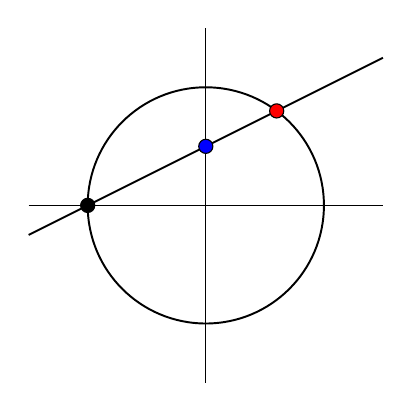
\begin{tikzpicture}[scale=1.5]
	\draw (-1.5,0) -- (1.5,0);
	\draw (0,-1.5) -- (0,1.5);

	\draw[line width=0.7] (-1.5,-0.25) -- (1.5,1.25);
	\draw[line width=0.7] (0,0) circle (1);
	
	\draw[fill=black] (-1,0) circle (0.06);
	\draw[fill=blue] (0,0.5) circle (0.06);
	\draw[fill=red] (0.6,0.8) circle (0.06);
	\end{tikzpicture}
	\] \vfill
	\[
	C(\Q)= \{ (-1,0) \} \cup \left\{ \left(\dfrac{1-t^2}{1+t^2}, \dfrac{2t}{1+t^2} \right) \colon t \in \Q \right\}
	\] \pspace
\end{frame}



% Empty Example
\begin{frame}[plain]
\frametitle{\textcolor{white}{$C(\Q)=\emptyset$}}

	\[
	x^2+y^2 + 1 = 0 
	\] \pspace

\begin{center} This has no real solutions: $C(\R)= \emptyset$ \end{center}
\end{frame}



% Empty Example 2
\begin{frame}[plain]
\frametitle{\textcolor{white}{$C(\Q)=\emptyset$}}

	\[
	x^2+y^2= 3 
	\] \pspace\pause

\begin{itemize}
\item Write $x=a/c$, $y=b/c$, and clear denominators to obtain
	\[
	a^2+b^2= 3c^2
	\] \pause

\item Now $a,b \in \Z$ are not both even, so $a^2 + b^2 \equiv 1 \mod 4$. But $2c^2 \equiv 0,2 \mod 4$.
\end{itemize}
\end{frame}



% Obstructions
\begin{frame}[plain]

\begin{prin}[Hasse, Local-Global Principle]
A collection of equations has a solution `if and only if' it has a solution in $\R$ and $\Q_p$ for all $p$.
\end{prin} \pspace \pause

\begin{itemize}
\item Not quite true---Selmer's Example: $3x^3+4y^3+5z^3=0$
\item The Hasse Principle shows that the only obstruction to rational points are essentially of one of the two previous forms. 
\end{itemize}

\end{frame}



% Higher Curves
\begin{frame}[plain]
\ctext{What about higher degree curves?}
\end{frame}



% Falting's Theorem
\begin{frame}[plain]

\begin{thm}[Mordell, 1922, Faltings, 1983]
If $C$ is a curve over $\Q$ of genus $g \geq 2$, then $C$ has at most finitely many rational points. 
\end{thm}
\end{frame}



% Sweet Spot
\begin{frame}[plain]

\ctext{This leaves the `sweet spot' of cubic equations}
\end{frame}



% Cubic Functions/Elliptic Curves
\begin{frame}[plain]
\frametitle{\textcolor{white}{$n=2, d=3$: $F(x,y)=0$}---Elliptic Curves}
	\[
	y^2 + a_1 xy + a_3y = x^3 + a_2 x^2 + a_4 x + a_6
	\] \pspace \pause

\begin{itemize}
\item Make the substitution $y \mapsto y + \dfrac{a_1 x+a_3}{2}$.
\item Obtain $y^2= x^3+ a_2' x^2 + a_4' x + a_6'$
\item Make the substitution $x \mapsto x + \dfrac{a_2'}{3}$
\end{itemize} \pspace \pause
	\[
	E_{A,B}: y^2 = x^3 + Ax + B
	\] \pspace

\begin{itemize}
\item Require $\Delta= -16(4A^3+27B^2) \neq 0$.
\item $C(\Q)$ could be empty, finite, or infinite. 
\end{itemize}
\end{frame}



% EC Definition
\begin{frame}[plain]
\begin{dfn}[Elliptic Curve]
An elliptic curve is\dots
\begin{itemize}
\item A nonsingular projective curve of genus 1.
\item An abelian variety of dimension 1.
\item A nonempty smooth variety, $V(F)$, with $\deg F=3$.
\item A compact Riemann surface of genus 1.
\item The set $\{(x,y) \colon y^2= x^3 + Ax + B, -16(4A^3+27B^2) \neq 0\} \cup \{\infty\}$ with an addition law given by the chord-tangent law. 
\end{itemize}
\end{dfn}
\end{frame}



% Examples 
\begin{frame}[plain]
	\begin{figure}[h]
	\centering
	\begin{subfigure}{0.45\textwidth}
	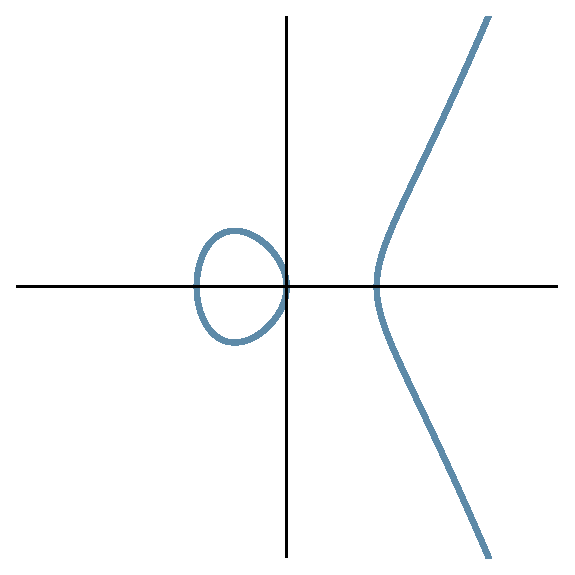
\includegraphics[width=\textwidth]{images/ec2.eps}
	\caption*{$y^2=x(x^2+1)$}
	\end{subfigure}
	%
	\begin{subfigure}{0.45\textwidth}
	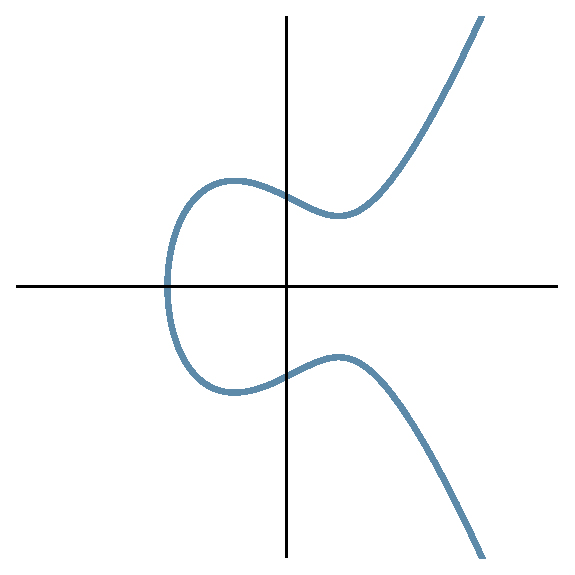
\includegraphics[width=\textwidth]{images/ec1.eps}
	\caption*{$y^2=x^3-x+1$}
	\end{subfigure}
	\end{figure}
\end{frame}



% Examples
\begin{frame}[plain]
	\begin{figure}
	\centering
	\begin{subfigure}{0.45\textwidth}
	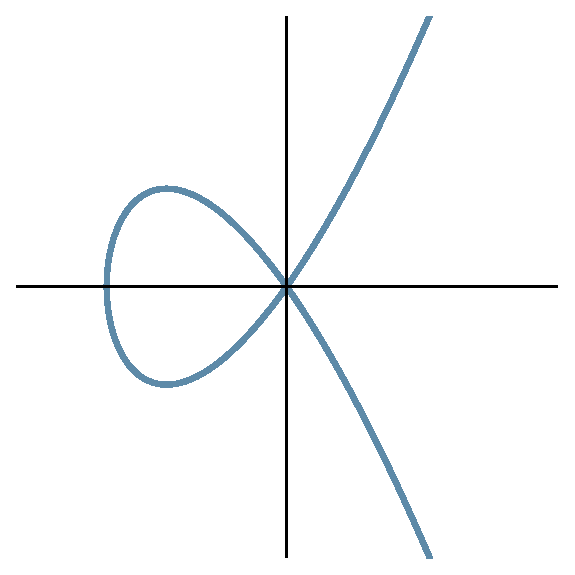
\includegraphics[width=\textwidth]{images/ec3.eps}
	\caption*{$y^2=x^2(x+2)$}
	\end{subfigure}
	\begin{subfigure}{0.45\textwidth}
	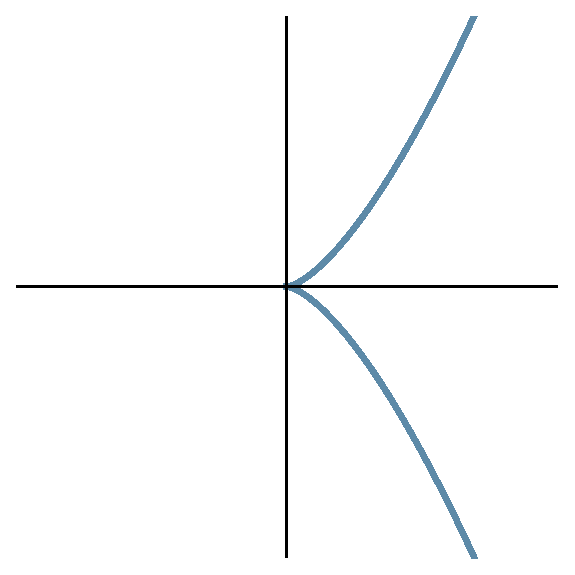
\includegraphics[width=\textwidth]{images/ec4.eps}
	\caption*{$y^2= x^3$}
	\end{subfigure}
	\end{figure}
\end{frame}



% Addition Law
\begin{frame}
	\begin{figure}[h]
	\centering
	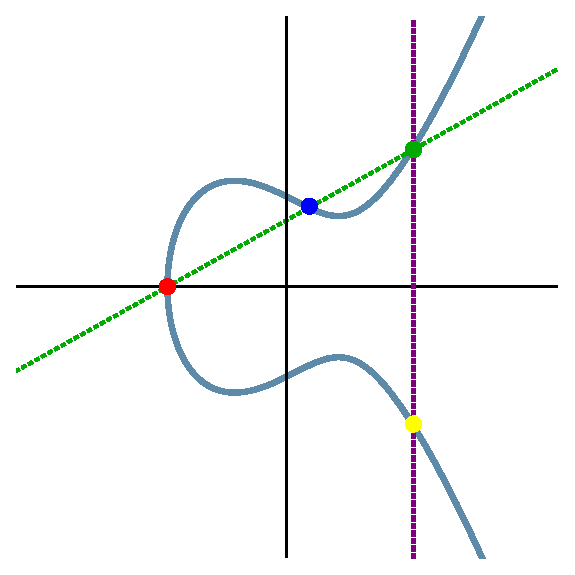
\includegraphics[width=0.75\textwidth]{images/ec_add.eps}
	\end{figure}
\end{frame}



% Complex Structure
\begin{frame}[plain]
\ctext{What is $E(\C)$?}
\end{frame}



% Modular Form
\begin{frame}
\begin{dfn}[Weakly Modular Form of Weight $k$]
Let $k$ be an integer. A meromorphic function $f: \mathcal{H} \to \C$ is weakly modular form of weight $k$ if
	\[
	f(\gamma(\tau))= (c\tau+d)^k f(\tau) \text{ for } \gamma= \begin{pmatrix} a & b \\ c & d \end{pmatrix} \in \text{SL}_2(\Z) \text{ and } \tau  \in \mathcal{H}
	\]
\end{dfn}

\begin{dfn}[Modular Form of Weight $k$]
Let $k$ be an integer. A function $f: \mathcal{H} \to \C$ is modular form of weight $k$ if

\begin{enumerate}[(i)]
\item $f$ is holomorphic on $\mathcal{H}$,
\item $f$ is weakly modular of weight $k$,
\item $f$ is holomorphic at $\infty$. 
\end{enumerate}
\end{dfn}

\end{frame}



% Complex Structure
\begin{frame}[plain]
\phantom{x} \par
Define the modular form, called the Weierstrass $\wp$-function,
	\[
	\wp(z)= \wp_\Lambda(z):= \dfrac{1}{z^2} + \sum_{\substack{\omega \in \Lambda \\ \omega \neq 0}} \left( \dfrac{1}{(z - \omega)^2} - \dfrac{1}{\omega^2} \right),
	\]
and define the Eisenstein series of weight $k$
	\[
	G_{k,\Lambda}= \sum_{\substack{\omega \in \Lambda \\ \omega \neq 0}} \omega^{-k}
	\]
$\wp(z)$ satisfies the following:
	\[
	\wp'(z)^2= 4\wp(z)^3 - 60G_4\wp(z) - 140 G_6
	\]
Now define an elliptic curve	
	\[
	\begin{aligned}
	y^2&= 4x^3 - g_2 x - g_3 \\
	g_2&= 60 G_4 \\
	g_3&= 140 G_6
	\end{aligned}
	\]
\end{frame}



% Isomorphism
\begin{frame}[plain]

\begin{thm}
Let $\Lambda$ be a lattice, and let $E$ be the elliptic curve $y^2= 4x^3 - g_2x - g_3$. Then
	\[
	\begin{aligned}
	\Phi: \C/\Lambda &\to E(\C) \\
	z &\mapsto (\wp(z),\wp'(z)) \\
	0 &\mapsto \infty
	\end{aligned}
	\]
is an isomorphism of groups.
\end{thm}
\end{frame}



% Other Direction
\begin{frame}[plain]
To go the other direction, write $E$ as 
	\[
	y^2= 4x^3 - g_2 x - g_3 = 4(x - e_1)(x - e_2)(x - e_3); \quad e_1<e_2<e_3
	\]
Then define
	\[
	\begin{aligned}
	\omega_1&= \dfrac{2i}{\sqrt{e_3-e_1} + \sqrt{e_3-e_2}} \int_1^{1/k} \dfrac{dt}{\sqrt{(t^2-1)(1-k^2t^2)}} \\
	\omega_2&= \dfrac{2}{\sqrt{e_3-e_1} + \sqrt{e_3-e_2}} \int_{-1}^1 \dfrac{dt}{\sqrt{(1-t^2)(1-k^2t^2)}}
	\end{aligned}
	\]
where
	\[
	k= \dfrac{\sqrt{e_3-e_1} - \sqrt{e_3-e_2}}{\sqrt{e_3-e_1} + \sqrt{e_3-e_2}}
	\] \pspace
Then $E(\C) \cong \C/\Lambda$, where $\Lambda= \Z \omega_1 + \Z\omega_2$.
\end{frame}



% Lattice
\begin{frame}[plain]
	\begin{figure}[!ht]
	\centering
	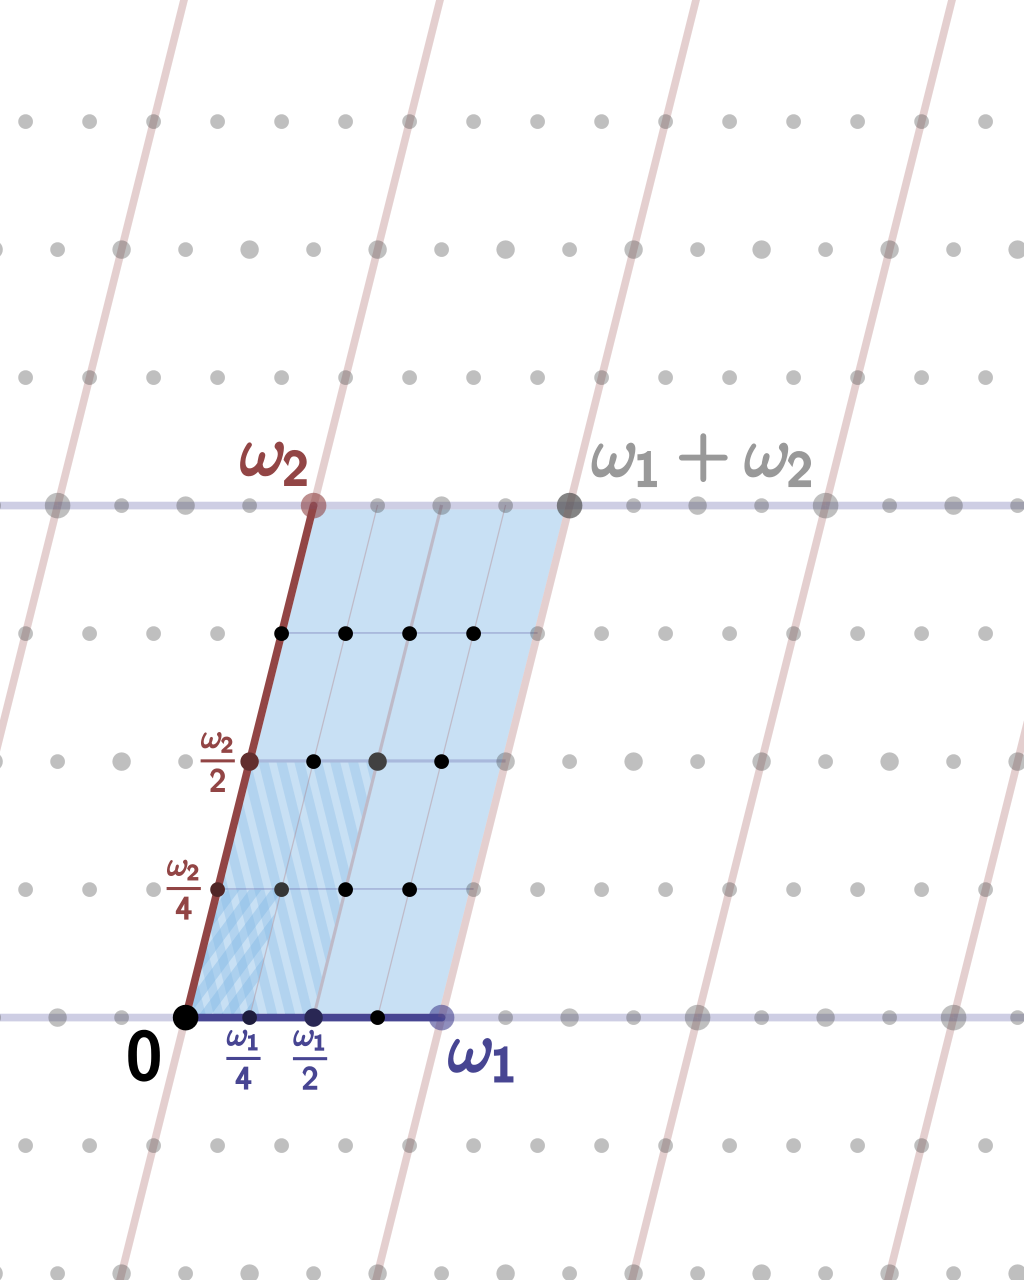
\includegraphics[width=0.7\textheight]{images/lattice.png}
	\end{figure}\fn{\tiny S. Derbyshire, \emph{Lattice torsion points}. CC BY-SA 3.0}
\end{frame}



% Lattice 2
\begin{frame}[plain]
	\begin{figure}[!ht]
	\centering
	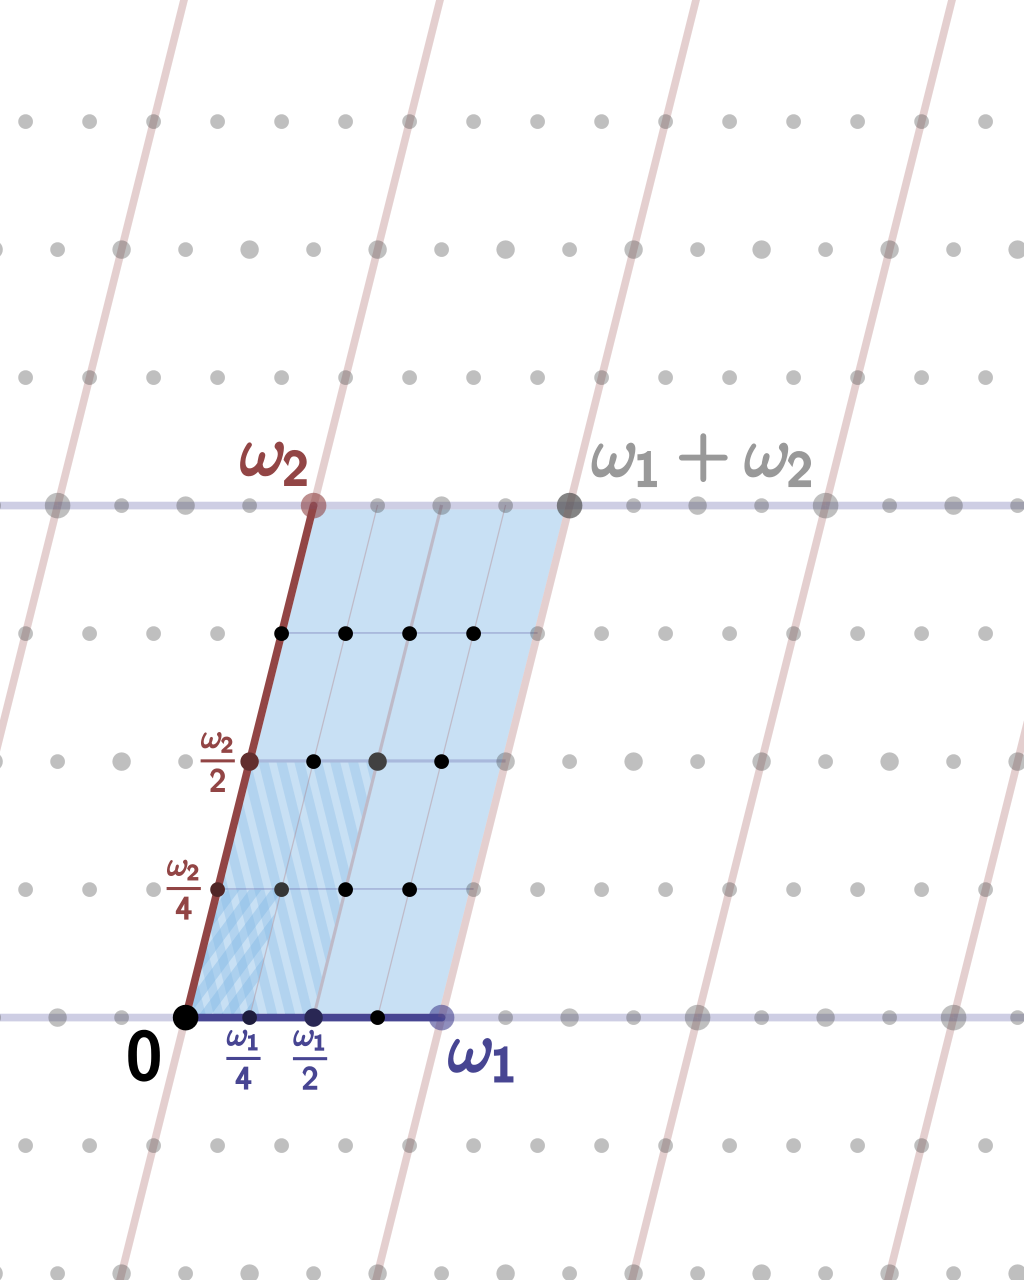
\includegraphics[width=0.3\textwidth]{images/lattice.png}
	\end{figure}

\begin{itemize}
\item This shows: $E[n]:= \{ P \in E \colon nP= \O \} \cong \Z/n\Z \oplus \Z/n\Z$
\item $E(\C)$ is isomorphic to a torus
	\begin{figure}[!ht]
	\centering
	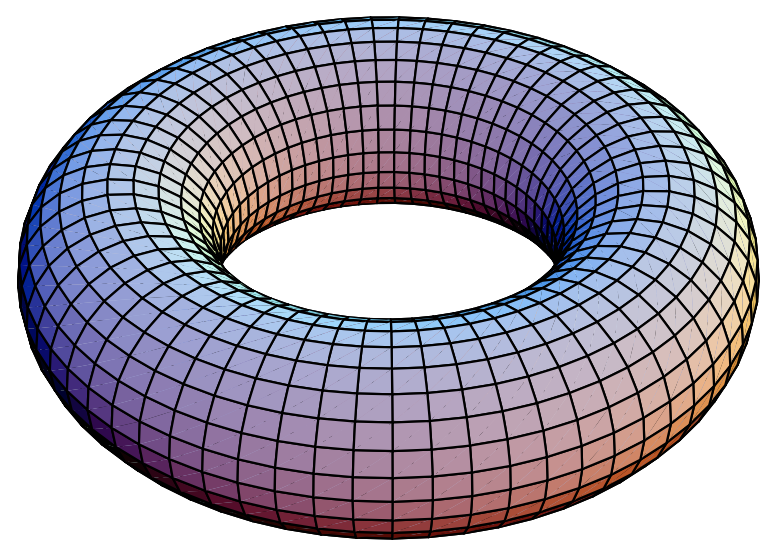
\includegraphics[width=0.3\textwidth]{images/torus.png}
	\end{figure}
\end{itemize}
\end{frame}



% E(R)
\begin{frame}[plain]
\ctext{What is $E(\R)$?}
\end{frame}



% E(R)
\begin{frame}[plain]
\phantom{x}\vfill
	\[
	E(\R) \cong S^1 \text{ or } E(\R) \cong S^1 \oplus \Z/2\Z
	\]
\vfill
\phantom{x}
\end{frame}



% Next
\begin{frame}[plain]
\ctext{The Structure of $E(\Q)$ in the next Talk\dots}
\end{frame}



% Odds 'N Ends
\begin{frame}[plain]
\ctext{Odd 'n Ends}
\end{frame}



% j-invariant
\begin{frame}[plain]
\frametitle{\textcolor{white}{$j$-invariant}}

Take an elliptic curve $y^2= x^3 + Ax + B$. The transformations which preserve this equations are: $x= \mu^2 x$ and $y= \mu^3 y$ for $\mu \in \overline{K}^\times$. We then define the $j$-invariant
	\[
	j= 1728 \dfrac{4A^3}{4A^4 + 27B^2}
	\]

These classify elliptic curves up to isomorphism over $\overline{K}$.

\begin{rem}
The $j$-invariant does not classify elliptic curves over $K$:
	\[
	\begin{aligned}
	y^2&= x^3 - 25x \\
	y^2&= x^3 - 4x
	\end{aligned}
	\]
Both have $j$-invariant 1728 but are not isomorphic over $K=\Q$ (but are over $K=\Q(\sqrt{10})$). So the $j$-invariant only classifies elliptic curves `up to twisting'. 
\end{rem}

\end{frame}



% Endomorphism Ring
\begin{frame}[plain]
\frametitle{\textcolor{white}{Endomorphism Ring}}

Considering the multiplication by $n$-map: $P \mapsto nP$
	\[
	\End E \supseteq \Z
	\]

Generally, $\End E$ is one of the following:
\begin{itemize}
\item $\Z$
\item an order in an imaginary quadratic field
\item an order in a quaternion algebra (not if $\char K= 0$)
\end{itemize}

If $\text{End }E \supsetneq \Z$, we say that $E$ has complex multiplication (CM). 

\begin{ex}
	\[
	\begin{aligned}
	y^2&= x^3 + B\\
	(x,y) &\mapsto (\zeta_3\, x,-y) \\
	y^2&= x^3 + Ax \\
	(x,y) &\mapsto (-x,iy)
	\end{aligned}
	\]
\end{ex}

% $\Aut E$ has order dividing 24, depening on $j$ and $\char K$, though it is typically 2, i.e. reflection across the $x$-axis.
\end{frame}



% Division Polynomials
\begin{frame}[plain]
\frametitle{\textcolor{white}{Division Polynomials}}
Consider an elliptic curve $y^2= x^3 + Ax + B$ and define
	\[
	\begin{aligned}
	\psi_0&= 0 \\
	\psi_1&= 1 \\
	\psi_2&= 2y \\
	\psi_3&= 3x^4 + 6Ax^2 + 12Bx - A^2 \\
	\psi_4&= 4y (x^6 + 5Ax^4 + 20Bx^3 - 5A^2x^2 - 4ABx - 8B^2 - A^3) \\
	&\vdots \\
	\psi_{2n+1}&= \psi_{n+2} \psi_n^3 - \psi_{n-2} \psi_{n+1}^3 \\
	\psi_{2n}&= \left(\dfrac{\psi_n}{2y}\right) (\psi_{n+2} \psi_{n-1}^2 - \psi_{n-2} \psi_{n+1}^2)
	\end{aligned}
	\]
The polynomial $\psi_n$ is called the $n$th division polynomial. The roots of $\psi_n$ give the $x$-coordinates of the $p$-torsion points. 
\end{frame}



% Weil Pairing
\begin{frame}[plain]
\frametitle{\textcolor{white}{Weil Pairing}}
There is a pairing $e_n: E[n] \times E[n] \to \Q(\zeta_n)$, called the Weil pairing, satisfying \pspace

\begin{enumerate}[(i)]
\item $e_n$ is bilinear
\item $e_n$ is non-degenerate 
\item $e_n(P,P)= 1$
\item $e_n(P,Q)= e_n(Q,P)^{-1}$
\item $e_n(P^\sigma,Q^\sigma)= \sigma e_n(P,Q)$ for all automorphisms of $\overline{K}$ which fix $A,B$.
\end{enumerate}

\begin{rem}
Using the Weil pairing, it is routine to verify that if $E[n] \subseteq K^2$, then $\Q(\zeta_n) \subseteq K$.
\end{rem}
\end{frame}



% Galois Representation
\begin{frame}[plain]
\frametitle{\textcolor{white}{Galois Representations}}

\begin{itemize}
\item Let $G_K:= \Gal(\overline{K}/K)$ be the absolute Galois group of $K$. 

\item $G_K$ acts on $E[n] \cong \Z/n\Z \oplus \Z/n\Z$

\item Fix a basis of $\Z/n\Z \oplus \Z/n\Z$, then we have a representation
	\[
	\rho_{E,n}: G_K \to \Aut(E[n]) \simeq \GL_2(\Z/n\Z),
	\]
the so-called mod $n$ Galois representation. 

\item One also forms the $\ell$-adic Tate module: $T_\ell(E):= \varprojlim_n E[\ell^n]$ and the $\ell$-adic representation $\rho_\ell: G_K \to \Aut(T_\ell(E))$. 
\end{itemize}

\begin{thm}[Serre]
Let $K$ be a number field, and let $E/K$ be an elliptic curve without CM. Then for all but finitely many primes $\ell$, $\rho_{E,\ell}: G_K \to \GL_2(\F_\ell)$ is surjective. 
\end{thm}
\end{frame}



% L-functions
\begin{frame}[plain]
\frametitle{\textcolor{white}{$L$-functions}}

Hasse Principle: $|p+1- \#E(\F_p)| \leq 2 \sqrt{p}$. We define `error terms' $a_p:= p + 1 - \#E(\F_p)$. \pause \par \vspace{0.5cm}

Then we define the Hasse-Weil $L$-function of $E$ to be
	\[
	L(E,s)= \prod_{p \nmid \Delta} \dfrac{1}{1 - a_p p^{-s} + p^{1-2s}}
	\] \pause
We can also write
	\[
	L(E,s)= \sum_{n \geq 1} \dfrac{a_n}{n^s},
	\]
where $a_n$ are the Fourier coefficients given by
	\[
	a_p=
	\begin{cases}
	p+1-N_p, & \text{if } E \text{ has good reduction at } p \\
	1, & \text{if } E \text{ has split multiplicative reduction at } p \\
	-1, & \text{if } E \text{ has non-split multiplicative reduction at } p \\
	0, & \text{if } E \text{ has additive reduction at } p
	\end{cases}
	\]
\end{frame}



% Modularity Theorem
\begin{frame}[plain]
\begin{thm}[Wiles, Taylor, Brueil, Conrad, Diamond]
$L(E,s)$ can be analytically continued to $\C$.
\end{thm}
	\begin{figure}[h]
	\centering
	\begin{subfigure}{0.3\textwidth}
	\captionsetup{labelformat=empty}
	\centering
	\fbox{
\includegraphics[width=0.6\textwidth]{images/wiles.jpg}}
	\caption{\scriptsize Andrew Wiles}
	\end{subfigure}
	%
	\begin{subfigure}{0.3\textwidth}
	\captionsetup{labelformat=empty}
	\centering
	\fbox{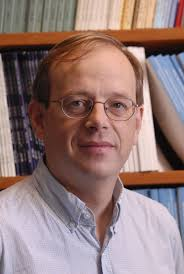
\includegraphics[width=0.43\textwidth]{images/taylor.jpeg}}
	\caption{\scriptsize Richard Taylor}
	\end{subfigure}
	%
	\begin{subfigure}{0.3\textwidth}
	\captionsetup{labelformat=empty}
	\centering
	\fbox{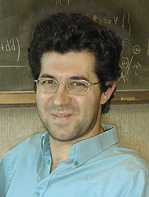
\includegraphics[width=0.5\textwidth]{images/breuil.jpg}}
	\caption{\scriptsize Christophe Breuil}
	\end{subfigure}
	%
	\\
	\begin{subfigure}{0.4\textwidth}
	\captionsetup{labelformat=empty}
	\centering
	\fbox{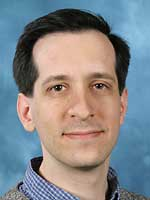
\includegraphics[width=0.35\textwidth]{images/conrad.jpg}}
	\caption{\scriptsize Brian Conrad}
	\end{subfigure}
	%
	\begin{subfigure}{0.4\textwidth}
	\captionsetup{labelformat=empty}
	\centering
	\fbox{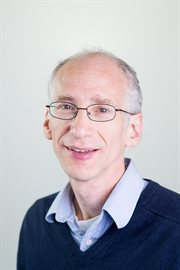
\includegraphics[width=0.35\textwidth]{images/diamond.jpg}}
	\caption{\scriptsize Fred Diamond}
	\end{subfigure}
	\end{figure}
\end{frame}



% Taylor Expansion
\begin{frame}[plain]
In particular, $L(E,s)$ has a Taylor expansion about $s=1$: \vspace{0.3cm}

	\[
	L(E,s)= c_0 + c_1 (s-1) + c_2(s-1)^2 + \cdots
	\] \pause \vspace{0.3cm}
	
Define the analytic rank $r_{an}$ of $E$ to be the order of vanishing of $L(E,s)$ at $s=1$, \vspace{0.3cm}

	\[
	L(E,s)= c_{r_{an}} (s - 1)^{r_{an}} + \cdots
	\] 
\end{frame}



% BSD
\begin{frame}[plain]

\begin{conj}[BSD]
The algebraic and analytic ranks of elliptic curves are equal.
\end{conj} 
	\begin{figure}[h]
	\centering
	\begin{subfigure}{0.3\textwidth}
	\captionsetup{labelformat=empty}
	\centering
	\fbox{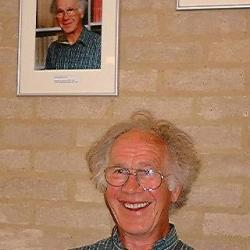
\includegraphics[width=0.7\textwidth]{images/birch.jpg}}
	\caption{Bryan Birch \\ \phantom{x}}
	\end{subfigure}
	%
	\begin{subfigure}{0.6\textwidth}
	\captionsetup{labelformat=empty}
	\centering
	\fbox{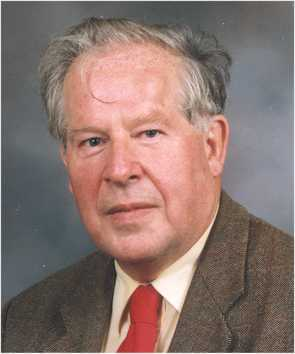
\includegraphics[width=0.3\textwidth]{images/dyer.jpg}}
	\caption{(Sir Henry) Peter \\ Francis Swinnerton-Dyer}
	\end{subfigure}
	\end{figure} \vspace{0.3cm}

\pause

Due to work of Gross, Zagier, Kolyvagin, if $r_{an} \leq 1$, then $r_{\text{anal}}=r_{alg}$.
If BSD is true, there is an algorithm to compute the rank of an elliptic curve. \pause

	\[
	\lim_{s \to 1} \dfrac{L(E,s)}{(s-1)^{r_E}} = \dfrac{\Omega_E \, \Reg(E) \, \#\sha(E/\Q) \, \prod_p c_p}{\#E(\Q)_{tors}^2}
	\]
\end{frame}



% Questions
\begingroup
\setbeamercolor{background canvas}{bg= gray, fg=white}
\begin{frame}[plain]
\phantom{x} \vfill
\begin{center} {\huge \textcolor{white}{Questions?}} \end{center}
\vfill
\end{frame}
\endgroup